% This file was created with tikzplotlib v0.10.1.
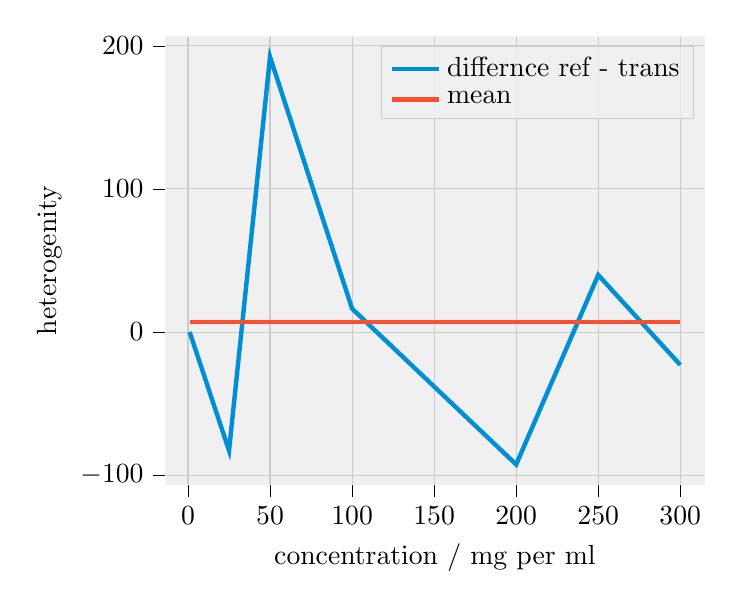
\begin{tikzpicture}

\definecolor{dodgerblue0143213}{RGB}{0,143,213}
\definecolor{lightgray203}{RGB}{203,203,203}
\definecolor{lightgray204}{RGB}{204,204,204}
\definecolor{tomato2527948}{RGB}{252,79,48}
\definecolor{whitesmoke240}{RGB}{240,240,240}

\begin{axis}[
axis background/.style={fill=whitesmoke240},
axis line style={whitesmoke240},
legend cell align={left},
legend style={fill opacity=0.8, draw opacity=1, text opacity=1, draw=lightgray204, fill=whitesmoke240},
tick align=outside,
tick pos=left,
x grid style={lightgray203},
xlabel={concentration / mg per ml},
xmajorgrids,
xmin=-13.95, xmax=314.95,
xtick style={color=black},
y grid style={lightgray203},
ylabel={heterogenity},
ymajorgrids,
ymin=-106.754044694627, ymax=206.463610538672,
ytick style={color=black}
]
\addplot [ultra thick, dodgerblue0143213]
table {%
1 0
25 -82.7207247281242
50 192.226444391703
100 16.3667181247976
200 -92.516878547659
250 39.8742977529615
300 -22.9351140053253
};
\addlegendentry{differnce ref - trans}
\addplot [ultra thick, tomato2527948]
table {%
1 7.18496328405058
25 7.18496328405058
50 7.18496328405058
100 7.18496328405058
200 7.18496328405058
250 7.18496328405058
300 7.18496328405058
};
\addlegendentry{mean}
\end{axis}

\end{tikzpicture}
